\subsection{UC2 - Sincronizzazione file da client a server}
\label{UC2}
\begin{figure}[H]
    \centering
    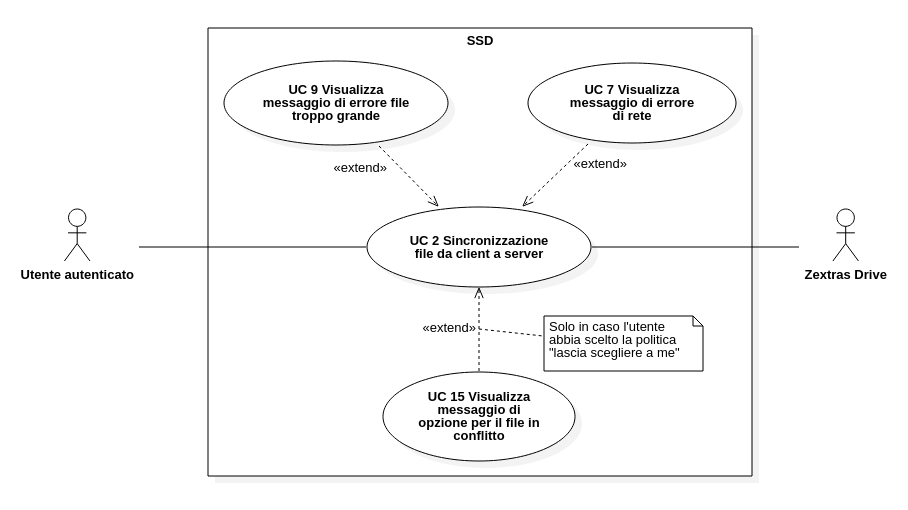
\includegraphics[scale = 0.7]{components/img/UC2.png}
    \caption{UC2 - Sincronizzazione file da client a server}
\end{figure}
\begin{itemize}
\item \textbf{Attore Primario:} Utente autenticato;
\item \textbf{Attore Secondario:} \glo{Zextras Drive};
\item \textbf{Precondizione:} L'utente ha la necessità di sincronizzare uno o più file, presenti nella cartella di root, dal client al server;
\item \textbf{Postcondizione:} L'utente ha sincronizzato i file presenti nella cartella di root dal client al server;
\item \textbf{Scenario principale:}
\begin{enumerate}
\item L'utente vuole sincronizzare dei file dal client verso il server;
\item Viene scelto dalla cartella di root l'insieme dei file che dovranno essere sincronizzati;
\item La sincronizzazione delle modifiche viene attivata per l'insieme scelto.
\end{enumerate}
\item \textbf{Estensioni:}
    \begin{itemize}
    \item Visualizza messaggio di errore file troppo grande (UC9 \S{}\ref{UC9});
    \item Visualizza messaggio di errore di rete (UC7 \S{}\ref{UC7}).
    \end{itemize}
\end{itemize}
